\begin{figure}[t]
\centering
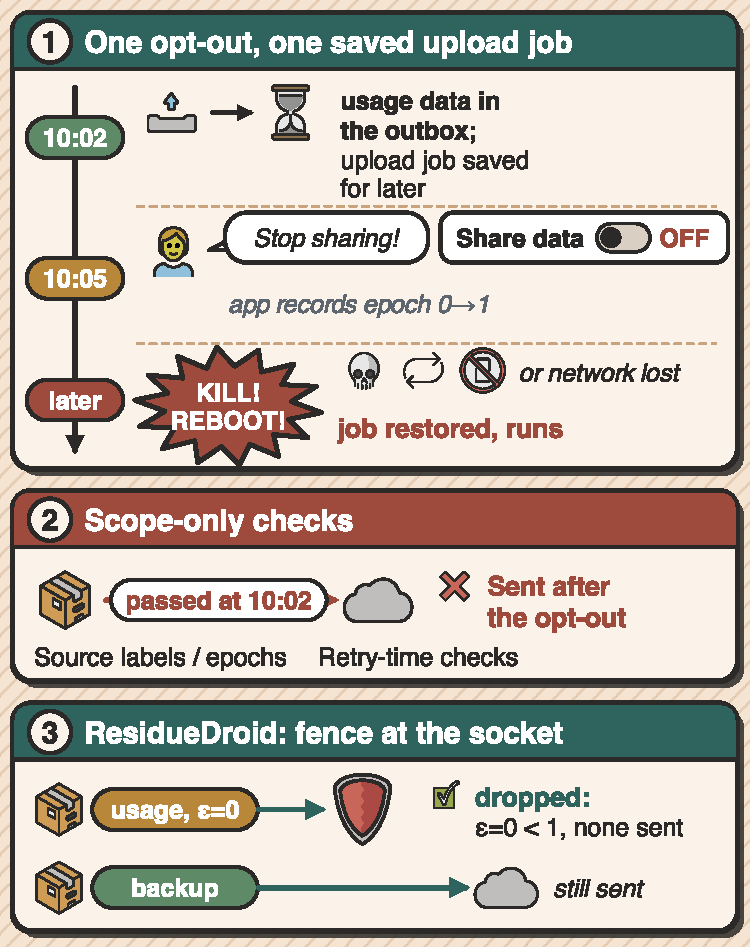
\includegraphics[width=\columnwidth]{figures/fig1.pdf}
\caption{(1)~A saved upload job outlives an opt-out across a kill, a reboot or a network loss. (2)~Checks made before submission let the data through. (3)~With \sys the label travels with the data and the fence at the socket drops it, while permitted flows such as backup still go out. Panel 2 names the information and retry checks needed by the fixture; it reports no population failure rate. Bytes already accepted before the opt-out are not recalled. Icons: OpenMoji (CC BY-SA 4.0).}
\Description{Comic with a vertical timeline panel and two stacked outcome panels. At 10:02 usage events and a summary go into an outbox and an upload job is saved; at 10:05 the user turns the Share data toggle off; later the process is killed, the device reboots or the network drops and the job is restored. With checks made earlier the data is sent after the opt-out. With ResidueDroid the labelled usage data is dropped at a fence at the socket while a backup flow is still sent.}
\label{fig:overview}
\end{figure}
